\chapter{Exercise 3}

\section{Implementation and thoughts behind}
\label{sec:detail_impl_analysisrunner}
In this section a detailed look into the chosen implementation 

\section{UML Class Diagram}
This section shows the the UML class diagramm for measuring the data in the data\_long.dat file. The whole code can be seen at \ref{sec:appendix_analysisrunner}. For a more detailed description of the classes \ref{sec:detail_impl_analysisrunner} is provided

\begin{landscape}
    \begin{figure}
        \begin{center}
            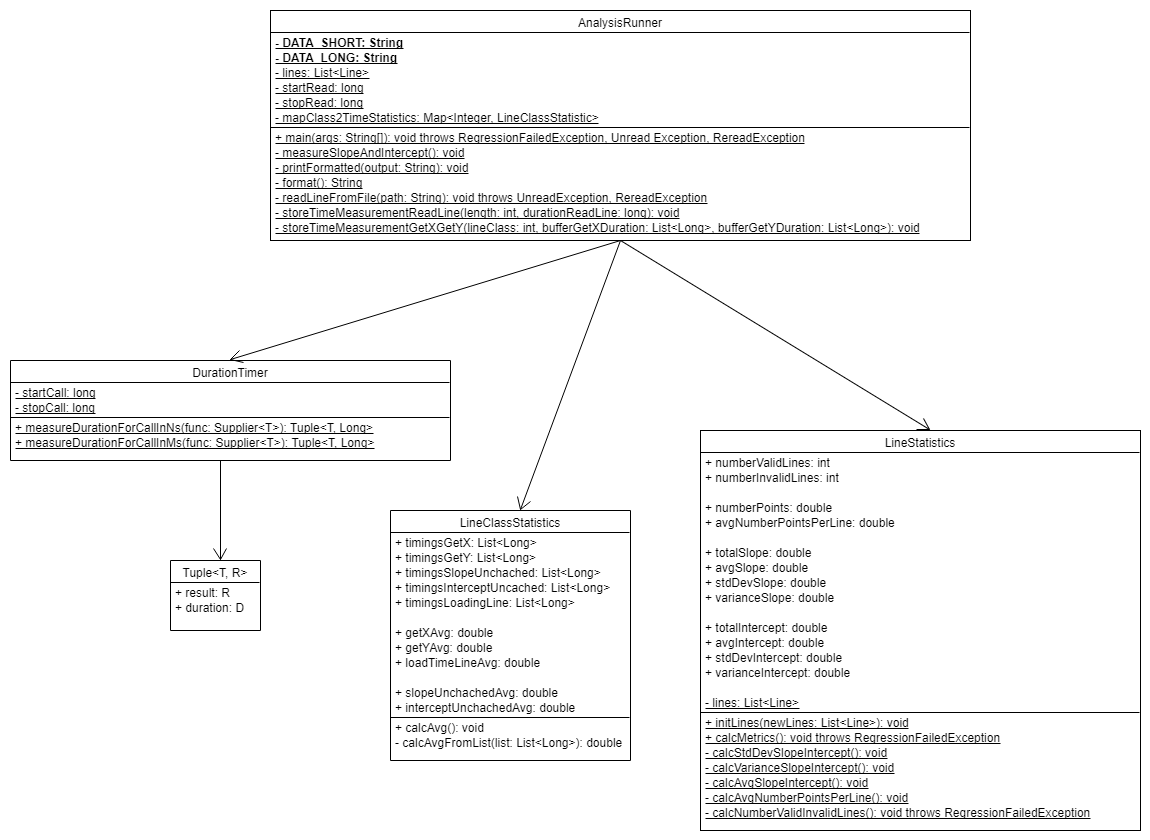
\includegraphics[width=1.45\textwidth]{img/classdiagram.png}
            \caption{UML class diagramm to measure timings}
        \end{center}
    \end{figure}
\end{landscape}